\documentclass[12pt,letterpaper, onecolumn]{exam}
\usepackage{amsmath}
\usepackage{amssymb}
\usepackage{sidecap}
\usepackage{tabularx}
\usepackage{csquotes}
\usepackage{makecell}
\usepackage{hyperref}
\hypersetup{
    colorlinks=true,
    linkcolor=blue,
    filecolor=magenta,      
    urlcolor=black,
    pdftitle={Overleaf Example},
    pdfpagemode=FullScreen,
}
%\usepackage[left=0.5cm,right=0.5cm,top=0.5cm,bottom=0.5cm]{geometry}
\usepackage[usestackEOL]{stackengine}
%\setstacktabbedgap{1ex} 
\usepackage{tikz}
\usetikzlibrary{decorations.pathreplacing}
\usetikzlibrary{fadings}
\def\layersep{2.5cm}

\usepackage{enumitem}
\usepackage{graphicx}

\usepackage{subcaption}

%\usepackage[shortlabels]{enumitem}
%\usepackage{enumerate}
\usepackage[lmargin=71pt, tmargin=0.8in]{geometry}  %For centering solution box

% \chead{\hline} % Un-comment to draw line below header
\thispagestyle{empty}   %For removing header/footer from page 1

\usepackage{listings}
\usepackage{xcolor}

\definecolor{codegreen}{rgb}{0,0.6,0}
\definecolor{codegray}{rgb}{0.5,0.5,0.5}
\definecolor{codepurple}{rgb}{0.58,0,0.82}
\definecolor{backcolour}{rgb}{0.95,0.95,0.92}

\lstdefinestyle{mystyle}{
    backgroundcolor=\color{backcolour},   
    commentstyle=\color{codegreen},
    keywordstyle=\color{magenta},
    numberstyle=\tiny\color{codegray},
    stringstyle=\color{codepurple},
    basicstyle=\ttfamily\footnotesize,
    breakatwhitespace=false,         
    breaklines=true,                 
    captionpos=b,                    
    keepspaces=true,                 
    numbers=left,                    
    numbersep=5pt,                  
    showspaces=false,                
    showstringspaces=false,
    showtabs=false,                  
    tabsize=2
}

\lstset{style=mystyle}




\begin{document}



\newtheorem{theorem}{Theorem}[section]
\newtheorem{problem}{Problem}
\newtheorem{proposition}{Proposition}[section]
\newtheorem{lemma}{Lemma}[section]
\newtheorem{corollary}[theorem]{Corollary}
\newtheorem{example}{Example}[section]
\newtheorem{definition}[problem]{Definition}

\newcommand{\BEQA}{\begin{eqnarray}}
\newcommand{\EEQA}{\end{eqnarray}}
\newcommand{\define}{\stackrel{\triangle}{=}}
\bibliographystyle{IEEEtran}
\raggedbottom
\setlength{\parindent}{0pt}
\providecommand{\mbf}{\mathbf}
\providecommand{\norm}[1]{\lVert#1\rVert}
\providecommand{\pr}[1]{\ensuremath{\Pr\left(#1\right)}}
\providecommand{\qfunc}[1]{\ensuremath{Q\left(#1\right)}}
\providecommand{\sbrak}[1]{\ensuremath{{}\left[#1\right]}}
\providecommand{\lsbrak}[1]{\ensuremath{{}\left[#1\right.}}
\providecommand{\rsbrak}[1]{\ensuremath{{}\left.#1\right]}}
\providecommand{\brak}[1]{\ensuremath{\left(#1\right)}}
\providecommand{\lbrak}[1]{\ensuremath{\left(#1\right.}}
\providecommand{\rbrak}[1]{\ensuremath{\left.#1\right)}}
\providecommand{\cbrak}[1]{\ensuremath{\left\{#1\right\}}}
\providecommand{\lcbrak}[1]{\ensuremath{\left\{#1\right.}}
\providecommand{\rcbrak}[1]{\ensuremath{\left.#1\right\}}}
\let\vec\mathbf

\newlist{mydesc}{description}{1} % create a new list called mydesc, of type "description"
\setlist[mydesc]{
  align=left, % use the align-format defined above
  leftmargin=0pt, % indentation for all the lines
  labelindent=1em, % horizontal space before label
  labelsep=0pt
   % horizontal space after label -- set to zero because we add space via "leftwithbar"
}



\begingroup  
    \centering
    
    \LARGE Weekly Report 2 - Naive Bayes\\[0.5em]
    
    \large Ganji Varshitha\par
    \large AI20BTECH11009\par
\endgroup
\rule{\textwidth}{0.4pt}
\pointsdroppedatright   %Self-explanatory
\printanswers
\newcommand\Solution{
  \textbf{Solution:}\\}
\newcommand{\myvec}[1]{\ensuremath{\begin{bmatrix}#1\end{bmatrix}}}
 %Replace "Ans:" with starting keyword in solution box

 \subsection*{Introduction}
Naive Bayes is a supervised learning algorithm which predicts the most probable class. It is very useful in text classification. Some of the applications include spam filtration, sentiment analysis, etc.

\subsection*{Why the name Naive Bayes?}
It is called Bayes because it estimates the bayesian probability of a class.\\
Let us assume a data point x has n features $A_1, A_2,\cdots A_n$. The posterior probability $P(C|A_1, A_2,\cdots A_n)$ where C denotes class is given by bayes theorem:
\begin{align}
P(C|A_1, A_2,\cdots A_n) = {}& \frac{P(A_1, A_2,\cdots A_n |C) P(C)}{P(A_1, A_2,\cdots A_n)}
\end{align}
It is naive because we assume independence of features $A_i$ when class is given.\\
This gives likelihood $P(A_1, A_2,\cdots A_n |C) = P(A_1|C) P(A_2|C) \cdots P(A_n|C)$.

\subsection*{Algorithm}
From the above theorem, we know that we should choose a class which maximises posterior probability i.e $P(C|A_1, A_2,\cdots A_n)$. \\
Since $P(A_1, A_2,\cdots A_n)$ is same for all values of C, we can omit the marginal probability.
\begin{align}
\hat{C} = \arg \max_{C} (P(A_1|C) P(A_2|C) \cdots P(A_n|C))P(C)
\end{align}
This is called Maximum A Posteriori estimation.\\
We also assume all the features contribute equally to the outcome.
\subsection*{Types of Naive Bayes Classifier}
\subsubsection*{Multinomial Naive Bayes}
It is mostly used in document classification where the feature values include the frequencies of words present in the document.
\subsubsection*{Bernoulli Naive Bayes}
It involves Bernoulli distribution. The feature values involve binary values. It is used in spam filtration and to find whether a word is present in the document.\\ The decision rule is based on
\begin{align}
P(x_i \mid y) = P(i \mid y) x_i + (1 - P(i \mid y)) (1 - x_i)
\end{align}
\subsubsection*{Gaussian Naive Bayes}
The feature values are continuous values and are assumed to be sampled from Gaussian distribution. We use maximum likelihood to estimate the parameters of the distribution with the given data. Using the probability distribution, conditional probability is given by
\begin{align}
P(x_i\mid y) = {}& \frac{1}{\sqrt{2\pi \sigma_y^2}}\exp\Big(-\frac{(x_i - \mu_y)^2}{2 \sigma_y^2}\Big)
\end{align}
\subsection*{Key points}
\begin{itemize}
\item The assumptions made in the algorithm does not always hold true in real-life problems.
\item It is robust to isolated noise points and irrelevant attributes.
\item To prevent floating point underflow, we sum logs of probabilities rather than multiplying.\\ Class with highest final un-normalized log probability score is still 
the most probable.
\item Algorithm gives probability distribution over all classes.
\item Since the algorithm is generative, we can handle missing data by ignoring the instance during probability estimation.
\end{itemize}
\subsection*{Questions}
\begin{questions}
\question[] Naive Bayes comes under \rule{2.5cm}{0.15mm} learning.
\begin{choices}
\choice Inductive
\choice Transductive
\end{choices}
\begin{Solution}
A. Inductive
\end{Solution}
\question[] Write the decision rule in terms of likelihood ratio for binary classification problem.
\begin{Solution}
\begin{align*}
g(x) ={}& \frac{P(C_1 \mid x)}{
P(C_2 \mid x) }\\
={}& 
\frac{P(x \mid C_1)P(C_1)}{P(x \mid C_2)P(C_2)}
\end{align*}
The decision rule is\\
choose $\begin{cases}
        C_1 & \text{if } g(x) > 1\\
        C_2 & \text{otherwise } 
    \end{cases}$



\end{Solution}
\question[] Is the model log linear?\\
\begin{Solution}
Yes.
\end{Solution}

\question[] Which of the following distribution has pdf?
\begin{choices}
\choice Bernoulli distribution
\choice Gaussian distribution
\end{choices}
\begin{Solution}
B. Gaussian distribution
\end{Solution}

\question[] Explain Bayesian networks.\\
\begin{Solution}
Bayesian network is a probabilistic graphical model that represents a set of variables and their conditional dependencies via a directed acyclic graph (DAG).
\begin{figure}[!h]
\centering
\begin{subfigure}{.5\textwidth}
  \centering
  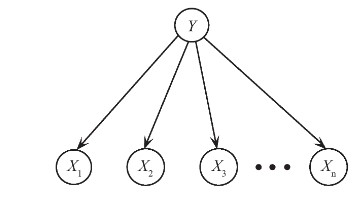
\includegraphics[width=.4\linewidth]{../images/Naive_bayes}
  \caption{Naive Bayesian network}

\end{subfigure}%
\begin{subfigure}{.5\textwidth}
  \centering
  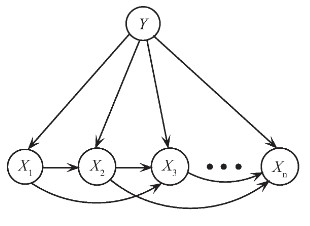
\includegraphics[width=.4\linewidth]{../images/Bayesian}
  \caption{Bayesian network with k dependencies}
\end{subfigure}
\end{figure}
\end{Solution}

\end{questions}



\end{document}